%%%%%%%%%%%%%%%%%Epic 4%%%%%%%%%%%%%%%%%%%%%%%%%%%%%%%%%%%%%%%%%%%%%%%%%%%%%%%
\subsection{Wegfindung}

In diesem Kapitel wird die Umsetzung der Wegfindung beschrieben. Ziel davon ist es, dass aufgrund von einem konfigurierten Graphen der schnellste Weg gefunden werden kann und die Kommunikation zwischen Navigation und Steuerung durchgeführt werden kann.

Das Finden des schnellsten Weg in einem Graphen wurde bereits in PREN 1 im Simulator umgesetzt mit einem Dijkstra Algorithmus. Der Simulator wird refactored, damit möglichst viele Teile wiederverwendet werden können.

\subsubsection{Wegfindungssoftware aus Simulator anpassen}
\label{navigation-arch}

Bevor der Simulator refactored wurde, wurde die neue Architektur designed für die Navigation, die auf Grafik \ref{fig:nav-arch} sichtbar ist.

\begin{figure}[H]
\centering
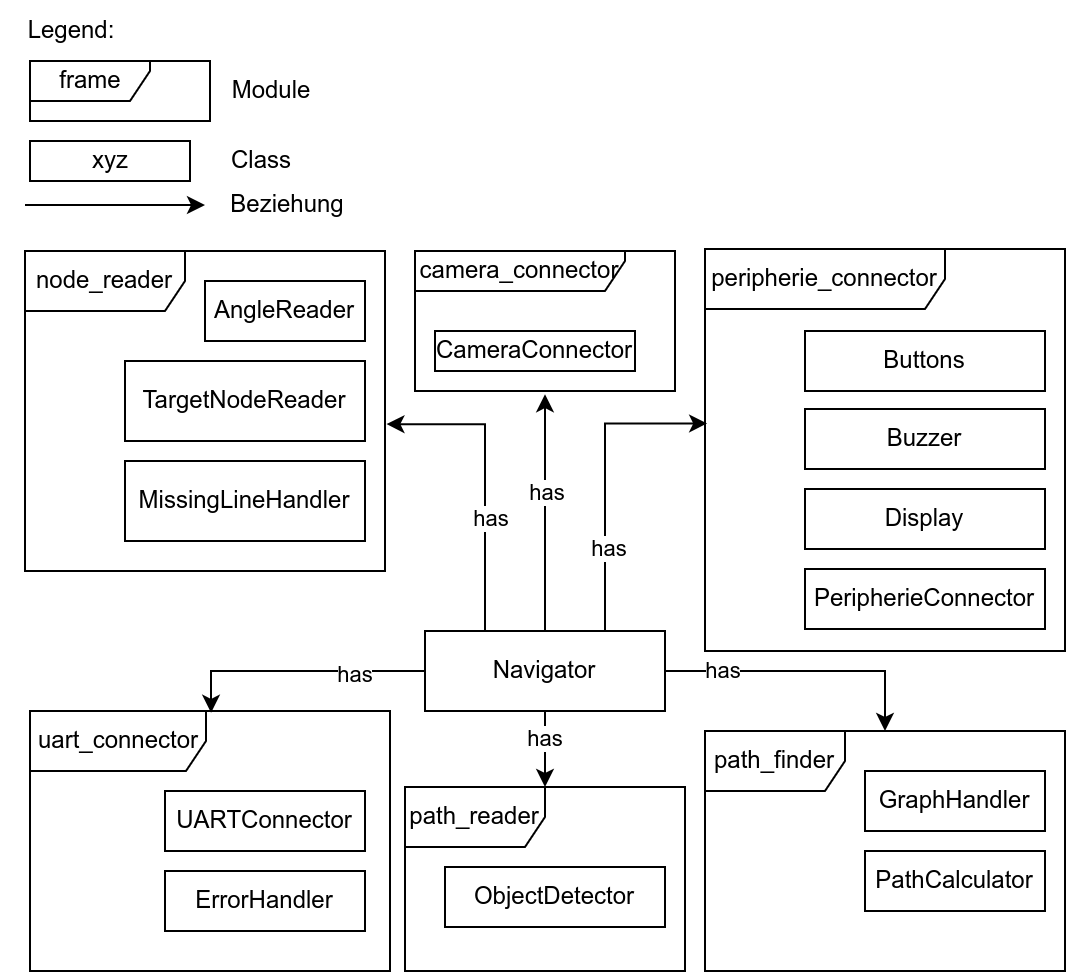
\includegraphics[width=\textwidth]{assets/IT/robot-sw-architecture-arch.png}
\caption{Aufbau Interface zu Steuerung}
\label{fig:nav-arch}
\end{figure}

Dieses Refactoring hilft dabei, dass strukturiert die simulierten Teile mit den realen Teilen ersetzt werden können und währenddessen sowohl auf einem Raspberry Pi, mit allen Verbindungen, als auch auf einem Laptop mit keinen Verbindungen eine lauffähige Version des Simulators verfügbar ist.
Durch verschiedene Environment Variablen\footnote{\url{https://de.wikipedia.org/wiki/Umgebungsvariable}} können die Hardware und der Funktionsumfang dynamisch gewählt werden. Nachfolgend in Tabelle \ref{table:environment-variables} sind diese Variablen ersichtlich


\begin{table}[H]
    \centering
    \begin{tabularx}{\textwidth}{|X|X|X|}
    \hline
        \textbf{Environment Variable} & \textbf{Beschreibung} & \textbf{Mögliche Werte}\\
        \hline
         \verb|PREN_PLATFORM| & Die Platform, auf welchem der Code ausgeführt wird. & \verb|PC| oder \verb|RPI| \\
         \hline
         \verb|PREN_CAMERA| & Die verwendete Kamera & \verb|NONE|, \verb|USB| oder \verb|PICAMERA| \\
         \hline
         \verb|PREN_UART| & Die verwendete Serielle Schnittstelle für die Kommunikation zwischen Raspberry Pi und \gls{tinyk22} & \verb|NONE| oder \verb|<DEVICE>| \newline (z.B. \verb|/dev/ttyAMA0|) \\
         \hline
         \verb|PREN_DISPLAY| & Das verwendete Display &  \verb|NONE|, \verb|OLED| oder \verb|TERMINAL|  \\
         \hline
    \end{tabularx}
    \caption{Environment Variabeln}
    \label{table:environment-variables}
\end{table}

Bei jedem Update wird getestet, ob die Version noch auf allen Plattformen lauffähig ist. Falls dies nicht der Fall wäre, kann durch die Benutzung von Git einfach auf eine alte Version zurück gewechselt werden. So muss das Risiko 14 von Software Updates, die Fehler mit sich bringen, nicht mehr beachtet werden.

Sowohl der Ablauf aus der Navigation selber die Berechnung der kürzesten Pfades und die interne Behandlung des Graphen sind gleicht wie in \acrshort{pren1} und sind auf den folgenden Grafiken \ref{fig:nav-navigator} und \ref{fig:nav-pathfinder} als Wiederholung gezeigt. Der Rest der einzelnen Module wird in den folgenden Kapiteln Schritt für Schritt im Detail aufgezeigt.

\begin{figure}[H]
  \centering
    \begin{minipage}[b]{0.48\textwidth}
    \centering
    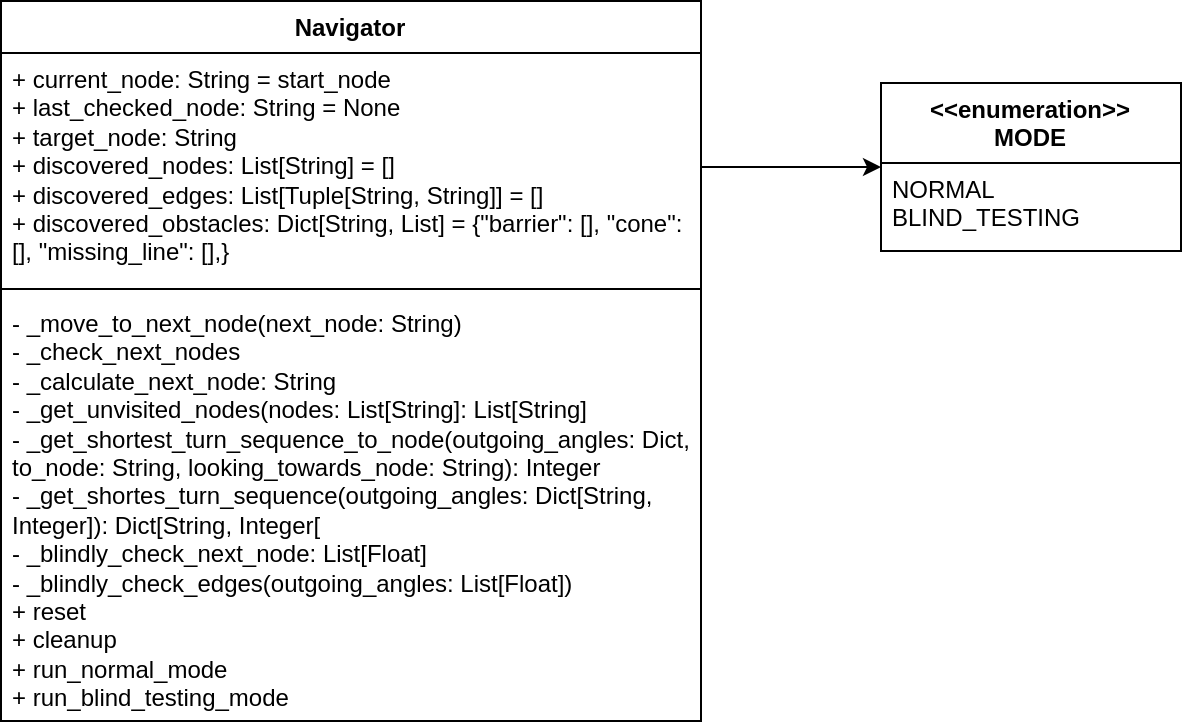
\includegraphics[width=\textwidth]{assets/IT/robot-sw-architecture-navigator.png}
    \caption{Navigator Modul}
    \label{fig:nav-navigator}
  \end{minipage}
  \hfill
  \begin{minipage}[b]{0.48\textwidth}
    \centering
    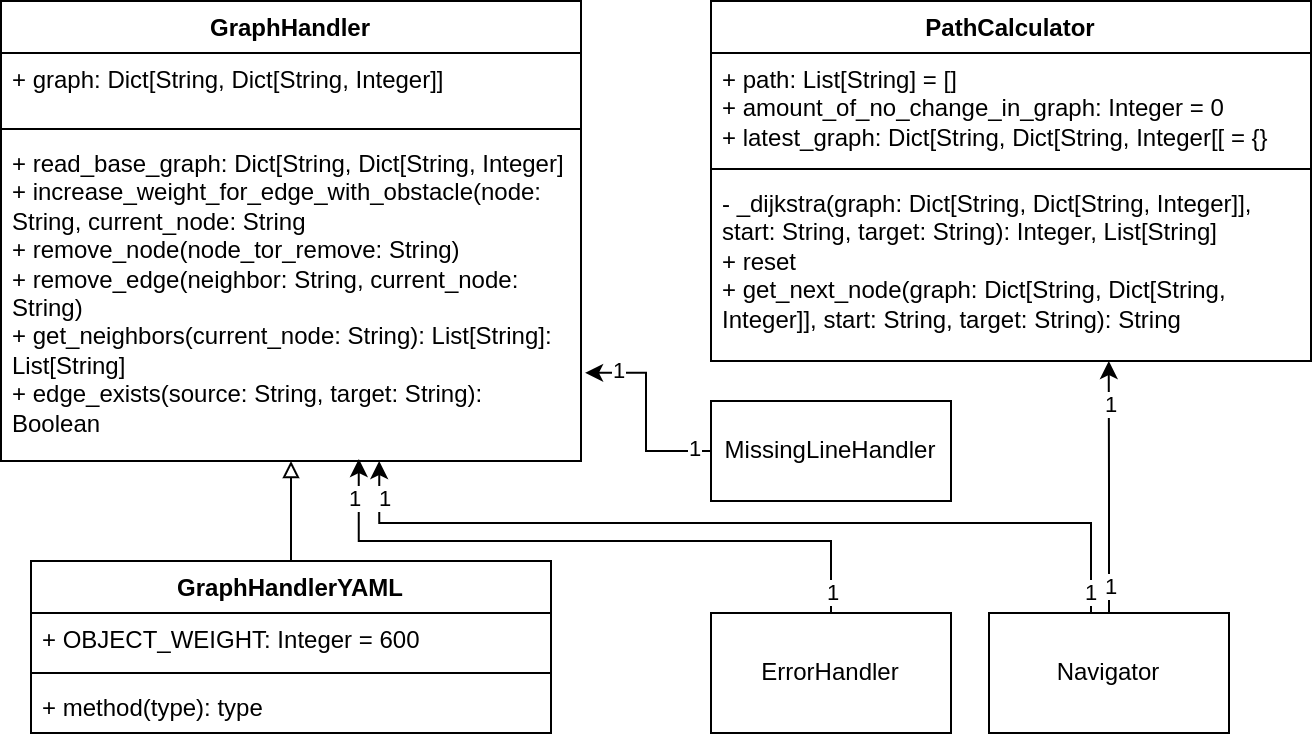
\includegraphics[width=\textwidth]{assets/IT/robot-sw-architecture-path_finder.png}
    \caption{Path Finder Modul}
    \label{fig:nav-pathfinder}
  \end{minipage}
\end{figure}

Ein grosser Unterschied von der neuen Architektur zu der Architektur des Simulators ist es, dass es eine klare Unterteilung in die einzelnen Module gibt, die die Navigation benötigt. So wird paralleles Arbeiten einfacher. Die Architektur modelliert nicht mehr die physischen Roboterteile, sondern nur noch die Navigationsteile.

Der gesamte Sourcecode zu der Navigation kann im Github-Repository (\url{https://github.com/ameyer3/hslu-pren-navigation}) oder im elektronischen Anhang gefunden werden.

Wie im Simulator aus \acrshort{pren1}, wird in der Navigation ein Trial \& Error Modus implementiert. Dieser Modus wird Blind Testing Mode genannt und wird eingeschaltet, falls es wirkt, als ob der Roboter nicht mehr weiss wo er sich befindet, beziehungsweise, falls er denkt er befindet sich auf einem anderen Knoten als er es tatsächlich tut. Die folgenden Situationen sind Zeichen, dass dies der Fall ist:

\begin{itemize}
    \item Roboter detektiert mehr ausgehenden Kanten von einem Knoten als erwartet.
    \item Falls in einem Winkelbereich, indem keine oder eine Kante erkannt werden soll, zwei Kanten erkannt werden.
    \item Falls der Dijkstra Algorithmus keine Route zum Ziel mehr findet.
\end{itemize}

Im Blind Testing Mode nimmt der Roboter jedes Mal die erste Kante von links, bei der keine Pylone erkannt wird und sucht so das Ziel. Obwohl es möglich ist, dass falsche Kanten entfernt werden und dies nicht auffällt, wird dies akzeptiert. Falls immer noch ein Weg gefunden kann, wird dieser zwar länger dauern, dies wird aber in Kauf genommen. Mit diesem Konzept können Risiko 20 (Roboter weiss nicht mehr wo er sich befindet) und Risiko 7 (Hindernis wird fälschlicherweise erkannt) so stark mitigiert werden, dass sie vernachlässigt werden können.

\subsubsection{Schnittstelle Navigation und Steuerung}
\label{interface-nav-control}

Die Navigation läuft auf einem Raspberry Pi und die Steuerung läuft auf einem \gls{tinyk22}. Die beiden kommunizieren wie geplant über das UART Protokoll miteinander. Für die Kommunikation wurde eine Schnittstelle definiert. Die Navigation sendet 4 Bytes an die Steuerung und die Steuerung antwortet mit dem Statuscode in Form von einem Byte.

Die Instruktionen von der Navigation an die Steuerung, werden, wie in Grafik \ref{fig:interface-tiny} gezeigt, gesendet.

\begin{figure}[H]
\centering
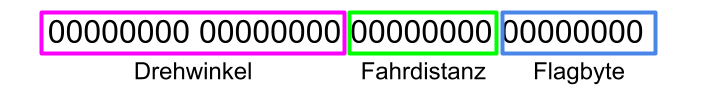
\includegraphics[width=\textwidth]{assets/IT/interface-tiny.png}
\caption{Aufbau Interface zu Steuerung}
\label{fig:interface-tiny}
\end{figure}

Die einzelnen Bytes sind in der folgenden Tabelle \ref{table:interface-to-tiny} beschrieben.

\begin{table}[H]
\centering
\small
\begin{tabularx}{\textwidth}{|c|c|X|}
\hline
  \textbf{Byte} &\textbf{Bezeichnung} & \textbf{Beschreibung}\\
  \hline
      1. Byte&1. Winkelbyte &Zeigt zusammen mit dem 2. Winkelbyte den Drehwinkel an. Die Steuerung addiert die beiden Werte und gibt den Befehl, dass der Roboter sich so weit drehen soll. In zwei Bytes aufgeteilt, da der Drehwinkel 255 übersteigen kann.\\
  \hline
2. Byte&2. Winkelbyte&Siehe 1. Winkelbyte.\\
  \hline
  3. Byte&Fahrbyte&Gibt die Distanz in Zentimeter an, die der Roboter fahren soll.\\
  \hline
  4. Byte&Flagbyte&Gibt an, ob der Roboter sich nach links oder rechts drehen soll, ob der Roboter vorwärts oder rückwärts fahren soll, ob sich eine Barriere auf der folgenden Strecke befindet.\\
  \hline
  \end{tabularx}
\caption{Interface zu Steurung}
\label{table:interface-to-tiny}
\end{table}

Die einzelnen Bedeutungen zu den Möglichkeiten des Flagbytes sind in Tabelle \ref{table:flag-to-tiny} erklärt.

\begin{table}[H]
\centering
\small
\begin{tabularx}{\textwidth}{|c|X|X|}
\hline
  \textbf{Flagbyte} & \textbf{Bedingung} & \textbf{Beschreibung}\\
  \hline
      0000&nur Winkelbyte gesetzt&Roboter soll sich nach links drehen.\\
  \hline
        0000&nur Fahrbyte gesetzt&Roboter soll vorwärts fahren.\\
  \hline
0001&nur Winkelbyte gesetzt&Roboter soll sich nach rechts drehen.\\
  \hline

0010&nur Fahrbyte gesetzt&Roboter soll rückwärts fahren.\\
  \hline

0100&kein zusätzliches Byte gesetzt&Auf folgender Strecke befindet sich eine Barriere.\\
  \hline
1000&kein zusätzliches Byte gesetzt&Roboter fährt bis er sich auf einem Knoten befindet.\\
  \hline
  \end{tabularx}
\caption{Flags in Interface zu Steurung}
\label{table:flag-to-tiny}
\end{table}



Die möglichen Statuscodes von der Steuerung an der Navigation sind in folgender Tabelle \ref{table:statuscodes} aufgelistet.

\begin{table}[H]
\centering
\small
\begin{tabularx}{\textwidth}{|c|l|X|}
\hline
  \textbf{Statusbyte} & \textbf{Encoding} & \textbf{Beschreibung} \\
  \hline
      00000000&SUCCESSFULLY\_DONE&Befehl wurde erfolgreich ausgeführt. \\
  \hline
00000001&UNEXPECTED\_OBJECT\_DETECTED &Ultraschall hat ein Objekt erkannt, das nicht erwartet wurde. Navigation macht ein Bild und detektiert, um welches Objekt es sich handelt und handelt entsprechend (mitigiert Risiko 12 (übersehene Objekte)): Kehrt um, falls Pylone oder beseitigt, falls Barriere.\\
  \hline
\end{tabularx}
\caption{Statuscodes von Steuerung}
\label{table:statuscodes}
\end{table}

\textbf{\gls{tinyk22} Implementation}

Für jedes empfangene Byte wird auf dem \gls{tinyk22} ein Interrupt generiert und anschliessend ausgelesen. Das Byte wird in einem Buffer Array zwischengespeichert. Nachdem die festgelegten 4 Bytes angekommen sind werden, die im Buffer zwischengespeicherten Bytes, in ein Array geschrieben. Aus diesem Array können dann die einzelnen Funktionen die nötigen Daten entnehmen und weiter verwenden.

\textbf{Raspberry Pi Implementation}

Auf dem Raspberry Pi wurde UART aktiviert, damit dieser mit dem \gls{tinyk22} kommunizieren kann.
Für die Kommunikation wird ein uart\_connector Modul erstellt. Dieses besteht aus der UARTConnector Klasse und der ErrorHandler Klasse, die die statische Methode 'handle\_errors' enthält. Auf folgender Grafik \ref{fig:uart-connector-nav} sind die beiden Klassen im Detail dargestellt mit ihrer Beziehung zu den anderen Klassen.

\begin{figure}[H]
\centering
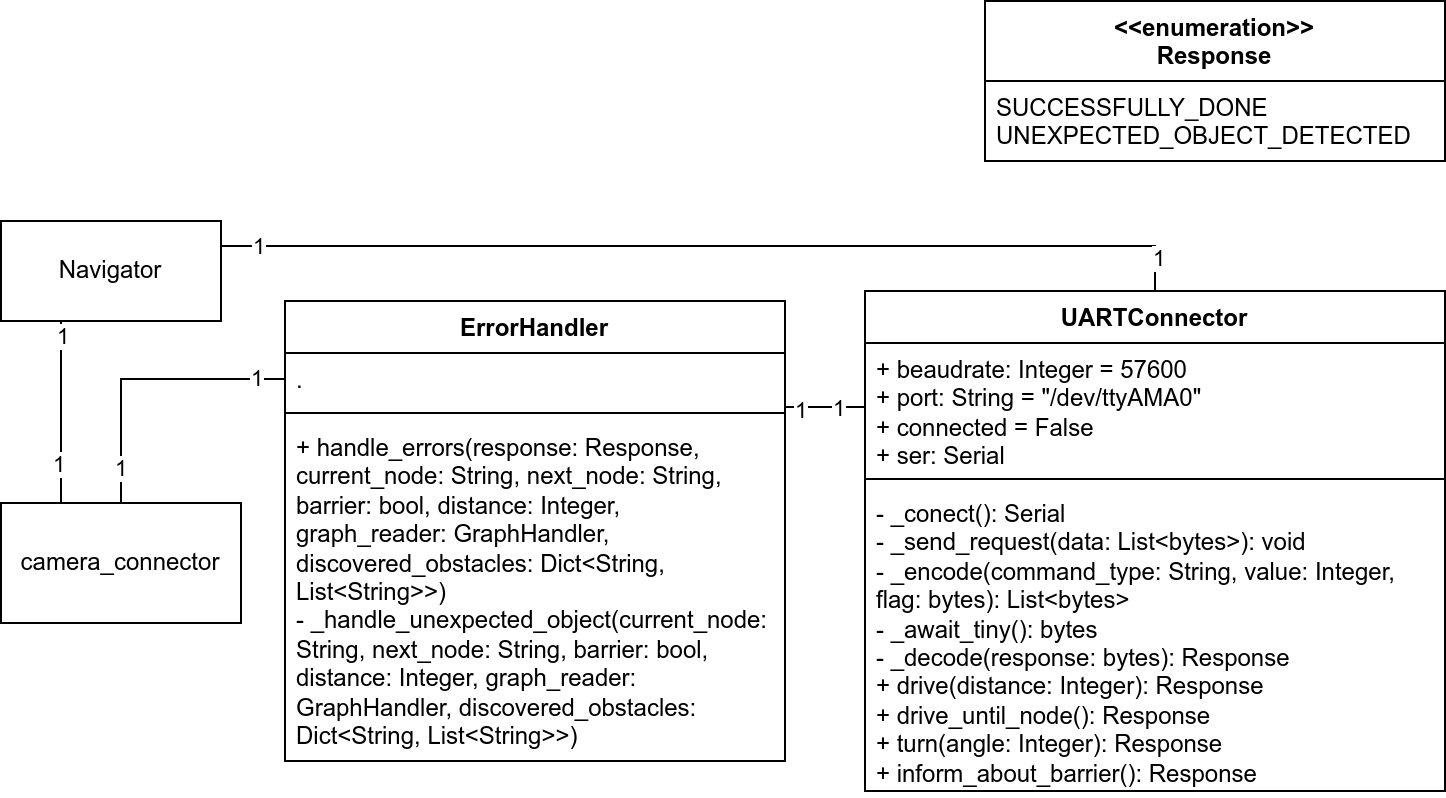
\includegraphics[width=\textwidth]{assets/IT/robot-sw-architecture-uart-connector.png}
\caption{UART Connector und Error Handler Klassendiagramm}
\label{fig:uart-connector-nav}
\end{figure}

Die UART-Connector Klasse  wird mithilfe der PySerial\footnote{\url{https://pypi.org/project/pyserial/}} Library implementiert. Diese kümmert sich selber um die Start- und Stop-Bits.
Die Verbindung wird mit diesen Zeilen aufgebaut:

\begin{verbatim}
beaudrate = 57600
port = "/dev/ttyAMA0"
self.ser = serial.Serial(self.port, self.beaudrate, timeout=1)
\end{verbatim}

Die Bewegungsinstruktionen werden, wie im Interface definiert, encoded. Es wird eine Liste mit 4 Bytes erstellt.
Diese Daten werden auf die serielle Verbindung geschrieben.
Danach wird gewartet, bis die Steuerung antwortet. Die Antwort wird wie in Tabelle \ref{table:statuscodes} decoded mit dem Response Enum.
Falls es einen 0 Statuscode (erfolgreich) gibt, wird normal weitergemacht. Falls ein andere Statuscode zurückgegeben wird, wird dieser dem ErrorHandler übergeben.

Der Errorhandler führt die Sequenz aus, die benötigt wird je nach Error.

Das Encoden der Nachrichten wurde mit mehreren Unittests getestet. Diese Unittests, sowie alle folgenden Unittests in der Navigation sind nach dem Muster `Arrange, Act, Assert'\footnote{\url{https://automationpanda.com/2020/07/07/arrange-act-assert-a-pattern-for-writing-good-tests/}} aufgebaut.

Im Arrange Teil wird hier festgelegt, was der Roboter machen soll und wie er antworten soll. Die Antwort wird gemocked\footnote{\url{https://microsoft.github.io/code-with-engineering-playbook/automated-testing/unit-testing/mocking/}} mithilfe von der Unittest Library.\footnote{\url{https://docs.python.org/3/library/unittest.mock.html}} Beispielsweise soll der Roboter -200cm fahren und die Antwort soll 0 sein, sprich, die Sequenz wurde richtig ausgeführt.

Im Act Teil wird die Funktion aufgerufen, die getestet wird. In diesem Beispiel ist das die `drive' Funktion.

Im Assert Teil wird getestet, ob die zurückgegebene Response korrekt decodiert wurde (von 0 zu SUCESSFULLY\_DONE) und ob die Funktion, die auf den \gls{tinyk22} schreibt, die richtigen Daten gesendet hat, was in diesem Fall ein Array mit folgendem Inhalt wäre:

\begin{verbatim}
# decimal values in Array get converted to Bytes when sent:
# 00000000, 00000000, 11001000 (200 to drive), 00000010 (drive backward)
[0, 0, abs(-200), 2]'
\end{verbatim}

Damit auch ohne Verbindung zu einem \gls{tinyk22} eine lauffähige Version verfügbar ist, wird beim Erstellen der UARTConnector Klasse geprüft, ob eine serielle Verbindung aufgebaut werden konnte. Wenn nicht, werden nach wie vor die alten Teile des Simulators verwendet. Dieser Zustand wird in der `connected' Variable festgehalten. Dies hilft beim Debuggen und Testen von einzelnen Modulen.


\newpage
%%%%%%%%%%%%%%%%%Epic 5%%%%%%%%%%%%%%%%%%%%%%%%%%%%%%%%%%%%%%%%%%%%%%%%%%%%%%%
\subsection{Hindernis umplatzieren}

Das Umplatzieren eines Hindernisses erfolgt in mehreren Stufen. Damit das Hindernis angehoben werden kann, wurde ein Greifer konstruiert und angebracht. Dies ist genauer aufgezeigt in Kapitel \ref{Greifer konstruieren}.

\subsubsection{Objekterkennung mit Ultraschall}

Die Barriere soll mit der Kamera erkannt werden, bevor der Roboter beginnt auf die Linie zu fahren. Der Raspberry Pi wird der Steuerung mitteilen, dass auf der nächsten Strecke eine Barriere zu erwarten ist. Der Roboter fährt dann langsamer als normalerweise los mit der Erwartung anzuhalten, wenn er 7cm vor sich das Objekt bemerkt. Diese Distanz sorgt dafür, dass sich der Roboter sicher drehen kann, ohne die Barriere umzustossen, jedoch die Distanz, die er langsam zum Hindernis zuruecklegt moeglichst kurz ist.

Falls die Kamera die Barriere nicht erkannt, aber trotzdem eine auf der Strecke ist, wird der Ultraschallsensor ein Objekt erkennen und der Navigation mitteilen, dass etwas im Weg steht. Die Navigation nutzt die Kamera, um herauszufinden, welches Objekt sich vor dem Roboter befindet. Wird dabei eine Barriere erkannt, fährt der Roboter noch naeher ran, um 7cm vor ihr zu sein und der Wegstell-Prozess wird gestartet, um das Hindernis aus dem Weg zu räumen. 

\subsubsection{Roboter drehen}

Der Roboter muss sich drehen können, um das Hindernis wegzustellen. Ebenfalls muss er sich drehen können, damit der Roboter sich ausrichten kann, um eine bestimmte Linie zu befahren. Die ist in dem folgenden Kapitel \ref{outgoing-lines} beschrieben.

In \acrshort{pren1} wurde geplant, dass der Roboter sich mit den Encodern dreht. Dabei sind jedoch immer wieder Probleme aufgetreten. Die Untersuchung davon ist im Anhang zu finden im Kapitel \nameref{drehen-encoder}.

Aus diesem Grund wurde entschieden ein Gyroskop zu verwenden.
 Ein Gyroskop reagiert auf Drehbewegungen, die durch die Corioliskraft verursacht wird. Die Corioliskraft bringt eine Masse ins Schwingen, so kann die Drehbewegung detektiert werden \parencite{zielke2025}. Dieser Sensor wird über \acrshort{iic} angesteuert, um die Messdaten auszulesen. 

Die Tests dazu sind im Anhang in Kapitel \nameref{drehen-gyro} zu finden. Nachdem die ersten Tests erfolgreich waren, wurde das Gyroskop fest auf den Roboter angeschlossen und montiert, wie in Abb. \ref{fig:Gyroskop auf dem Roboter} unten links zu sehen ist. Danach wurden Tests durchgeführt, ob das Gyroskop noch immer richtig misst, wenn der Roboter mit den Rädern und dem Motor dreht. Dies war erfolgreich.


\begin{figure}[H]
\centering
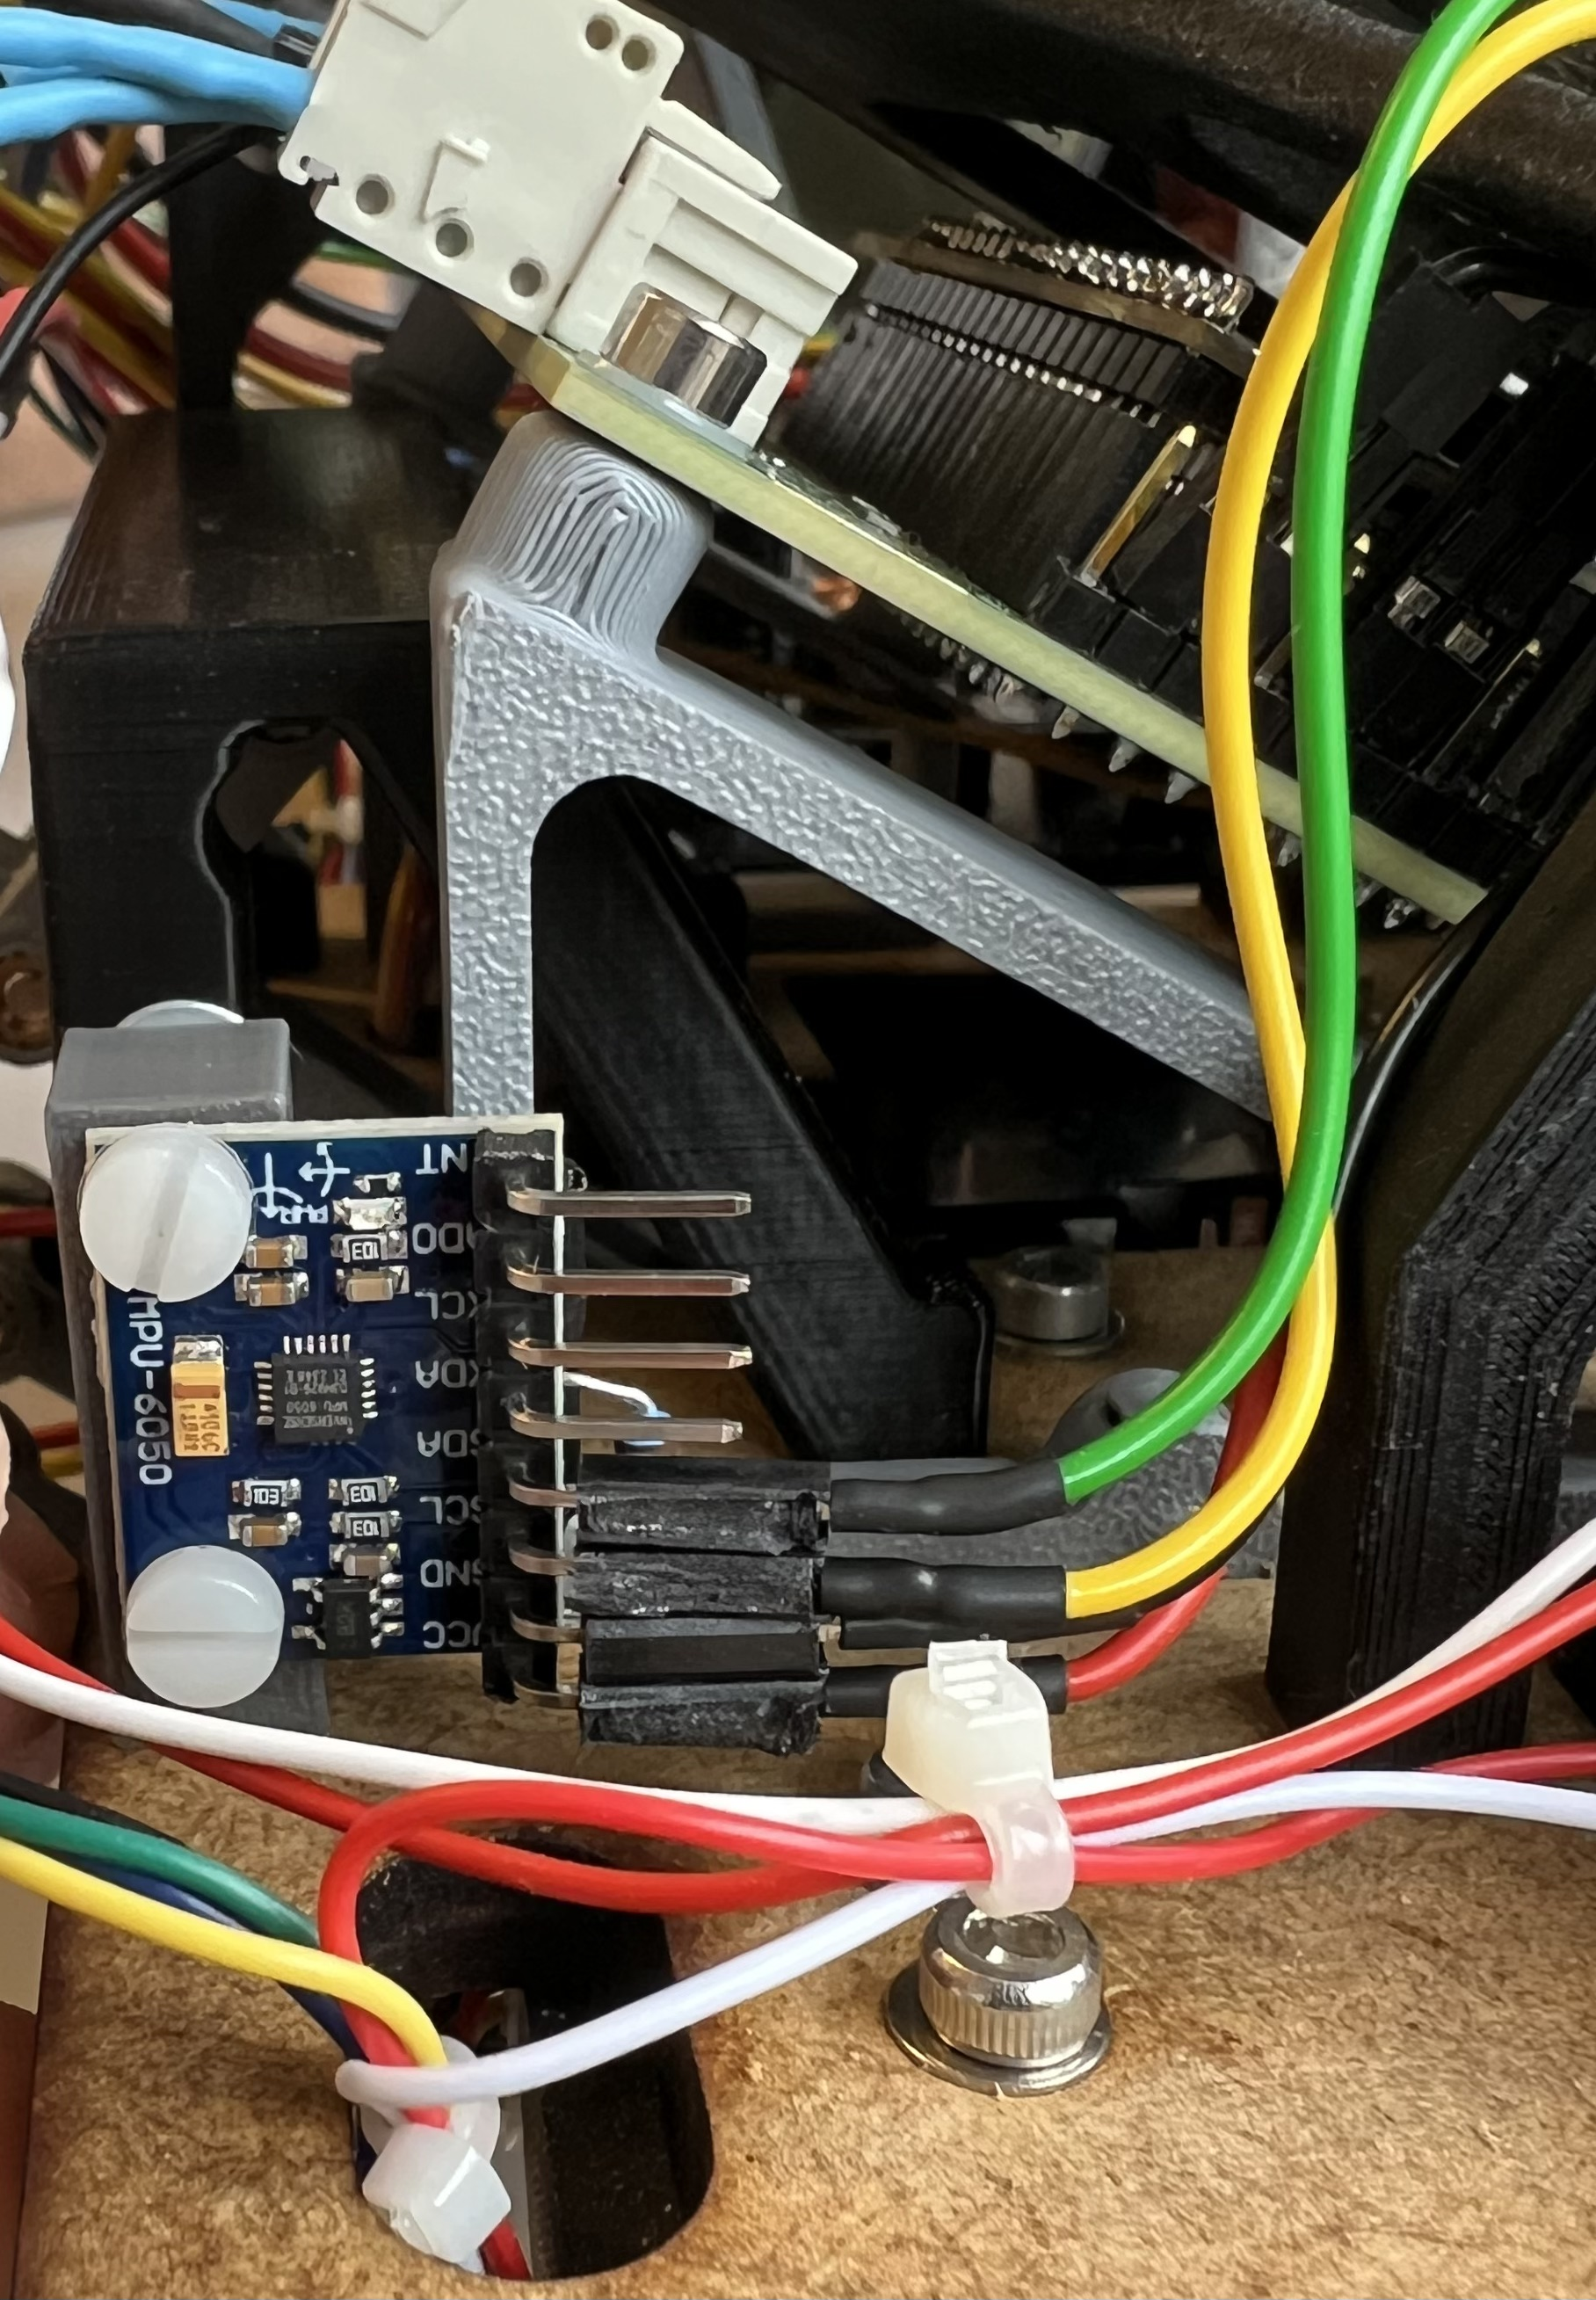
\includegraphics[width=5cm, height=7cm]{assets/ET/Gyroskop/Gyro_Montiert.jpeg}
\caption{Festmontierter Gyroskop auf dem Roboter}
\label{fig:Gyroskop auf dem Roboter}
\end{figure}

Es kann ein Befehl an die Steuerung gegeben werden mit dem gewünschten Winkel, in dem der Roboter sich drehen soll. Der Roboter dreht sich so lange, bis das Gyroskop misst, dass der Wert erreicht wurde, dann stoppt er.


\subsubsection{Servomotor für Greifer} 

Der Servomotor wurde bereits in Pren 1 getestet und dokumentiert. Durch die Ergebnisse von diesem Test konnte die Software erfolgreich implementiert werden.

\begin{figure}[H]
\centering
\begin{minipage}[b]{0.49\textwidth}
  \centering
    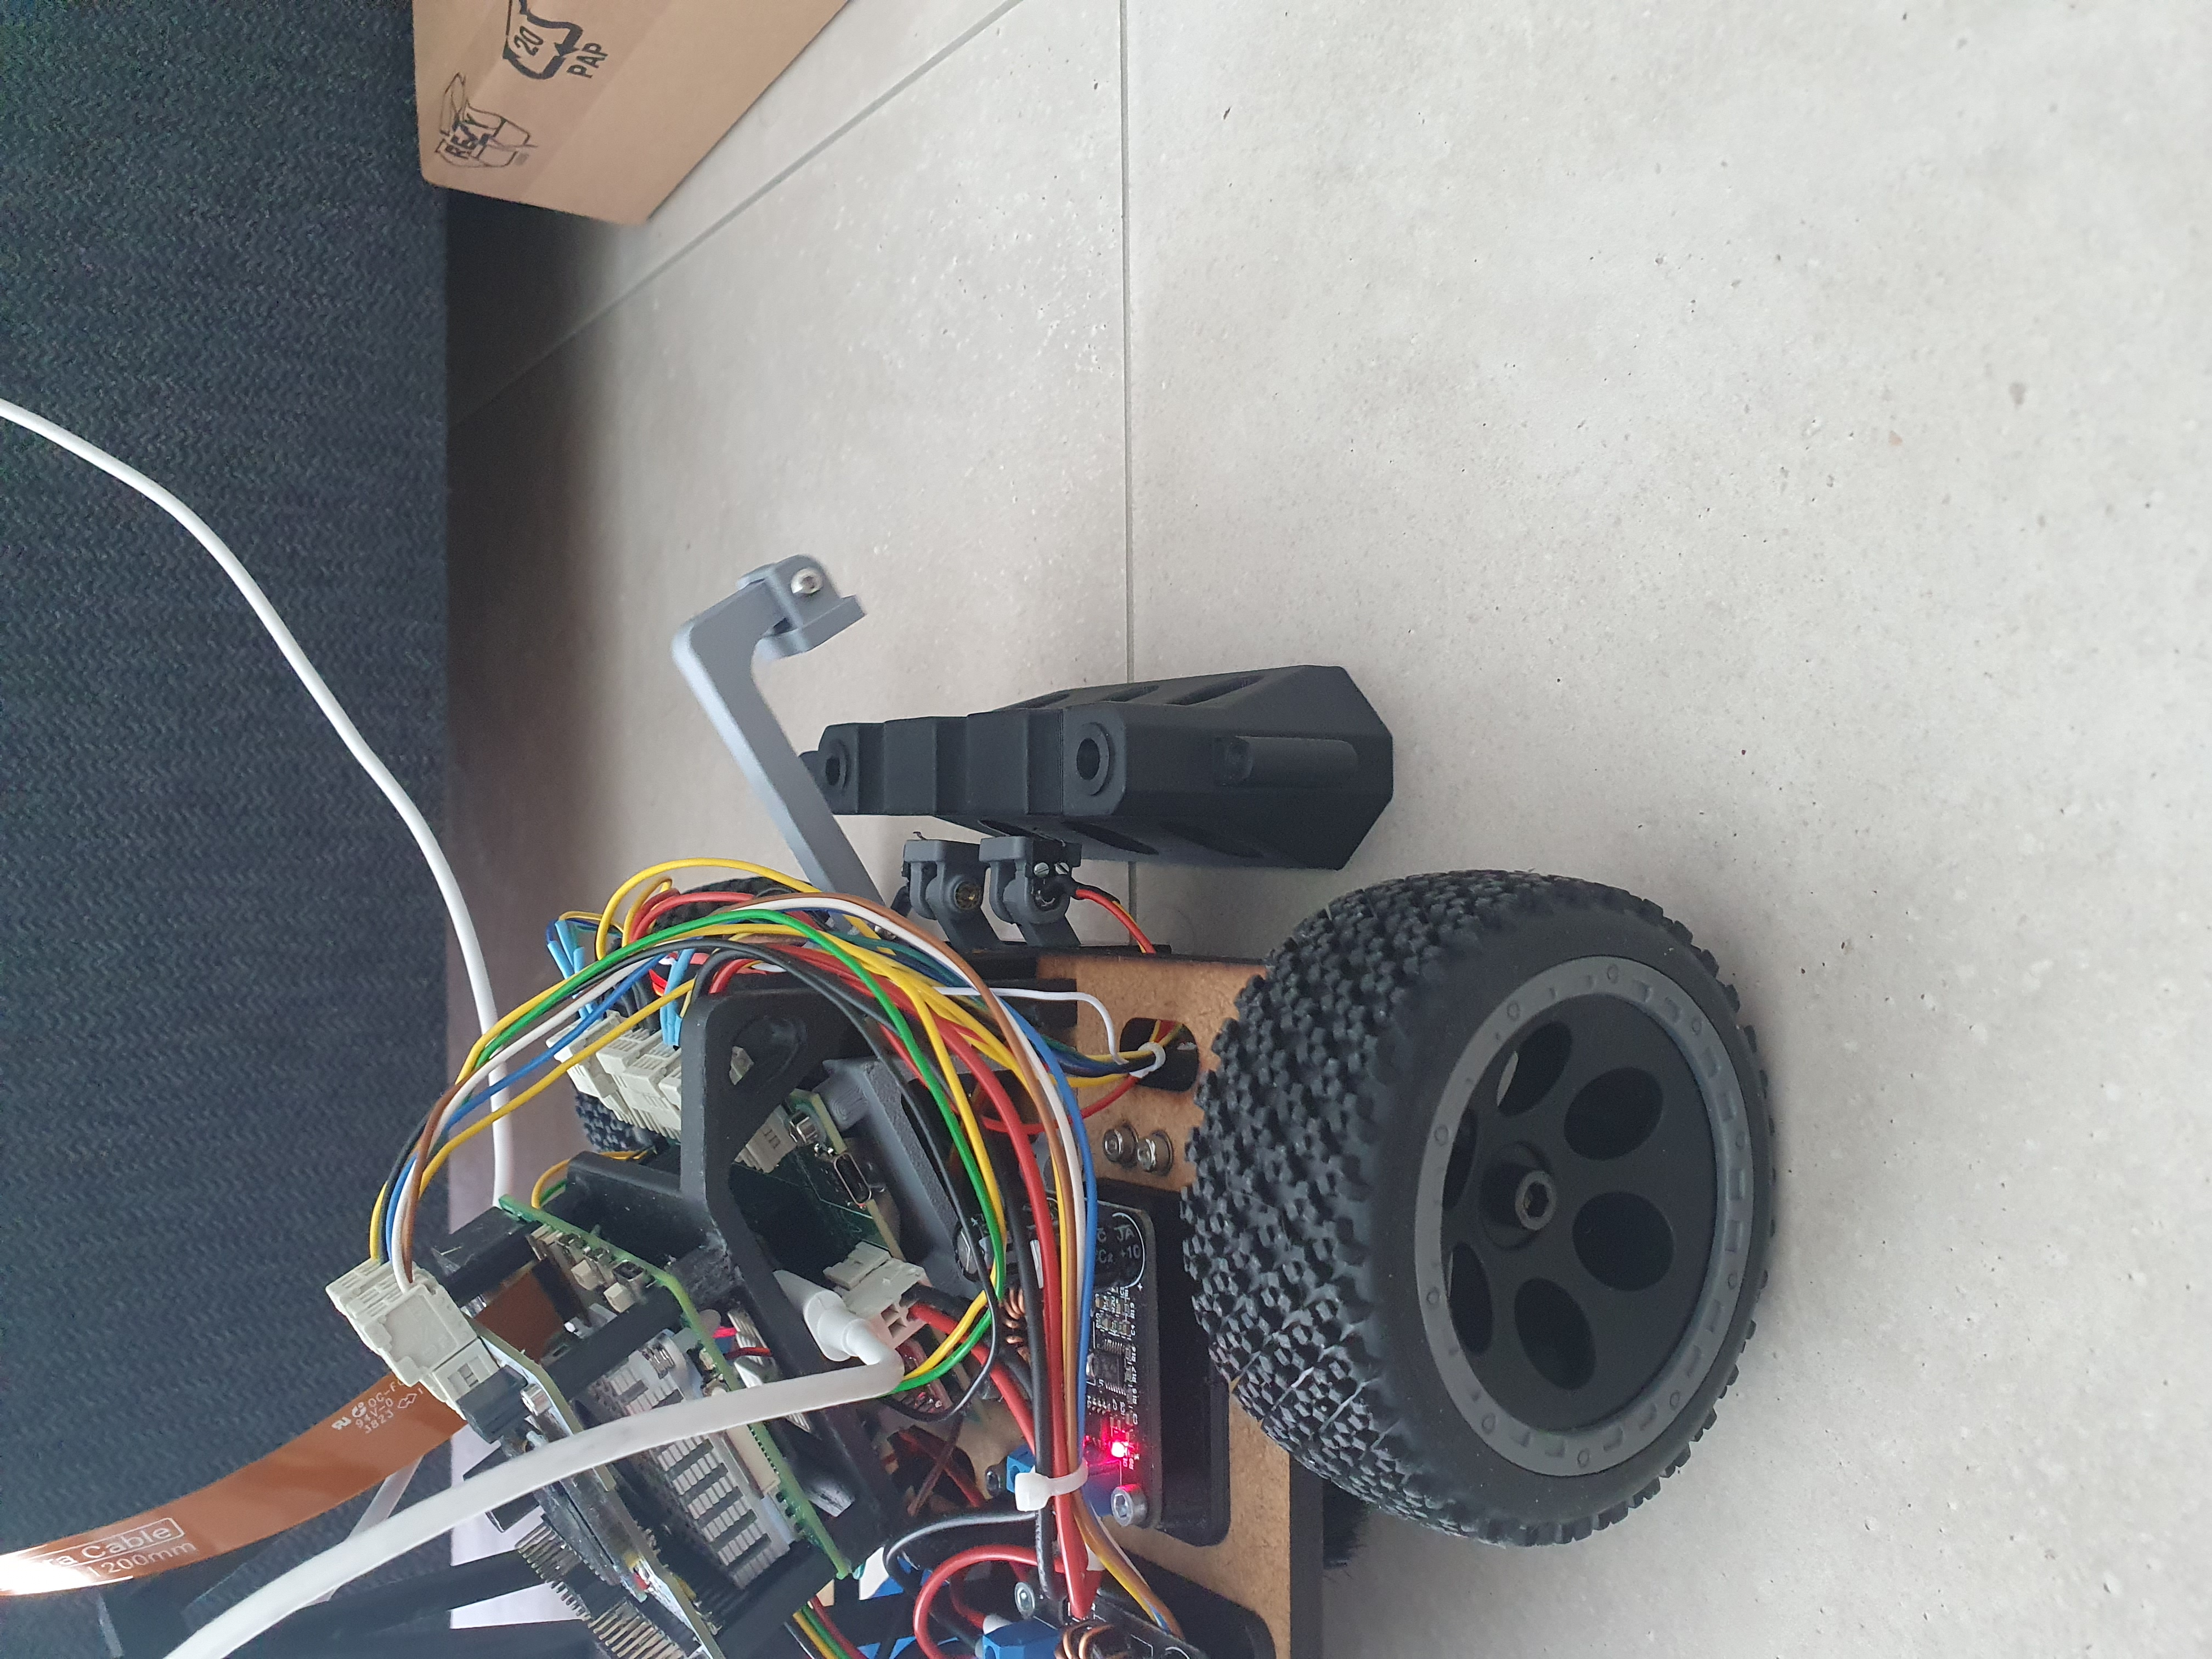
\includegraphics[width=\textwidth, angle=-90]{assets/MT/greifer-open.jpg}
    \caption{Greifer offen}
    \label{fig:greifer-open1}
\end{minipage}
\hfill
\begin{minipage}[b]{0.49\textwidth}
  \centering
  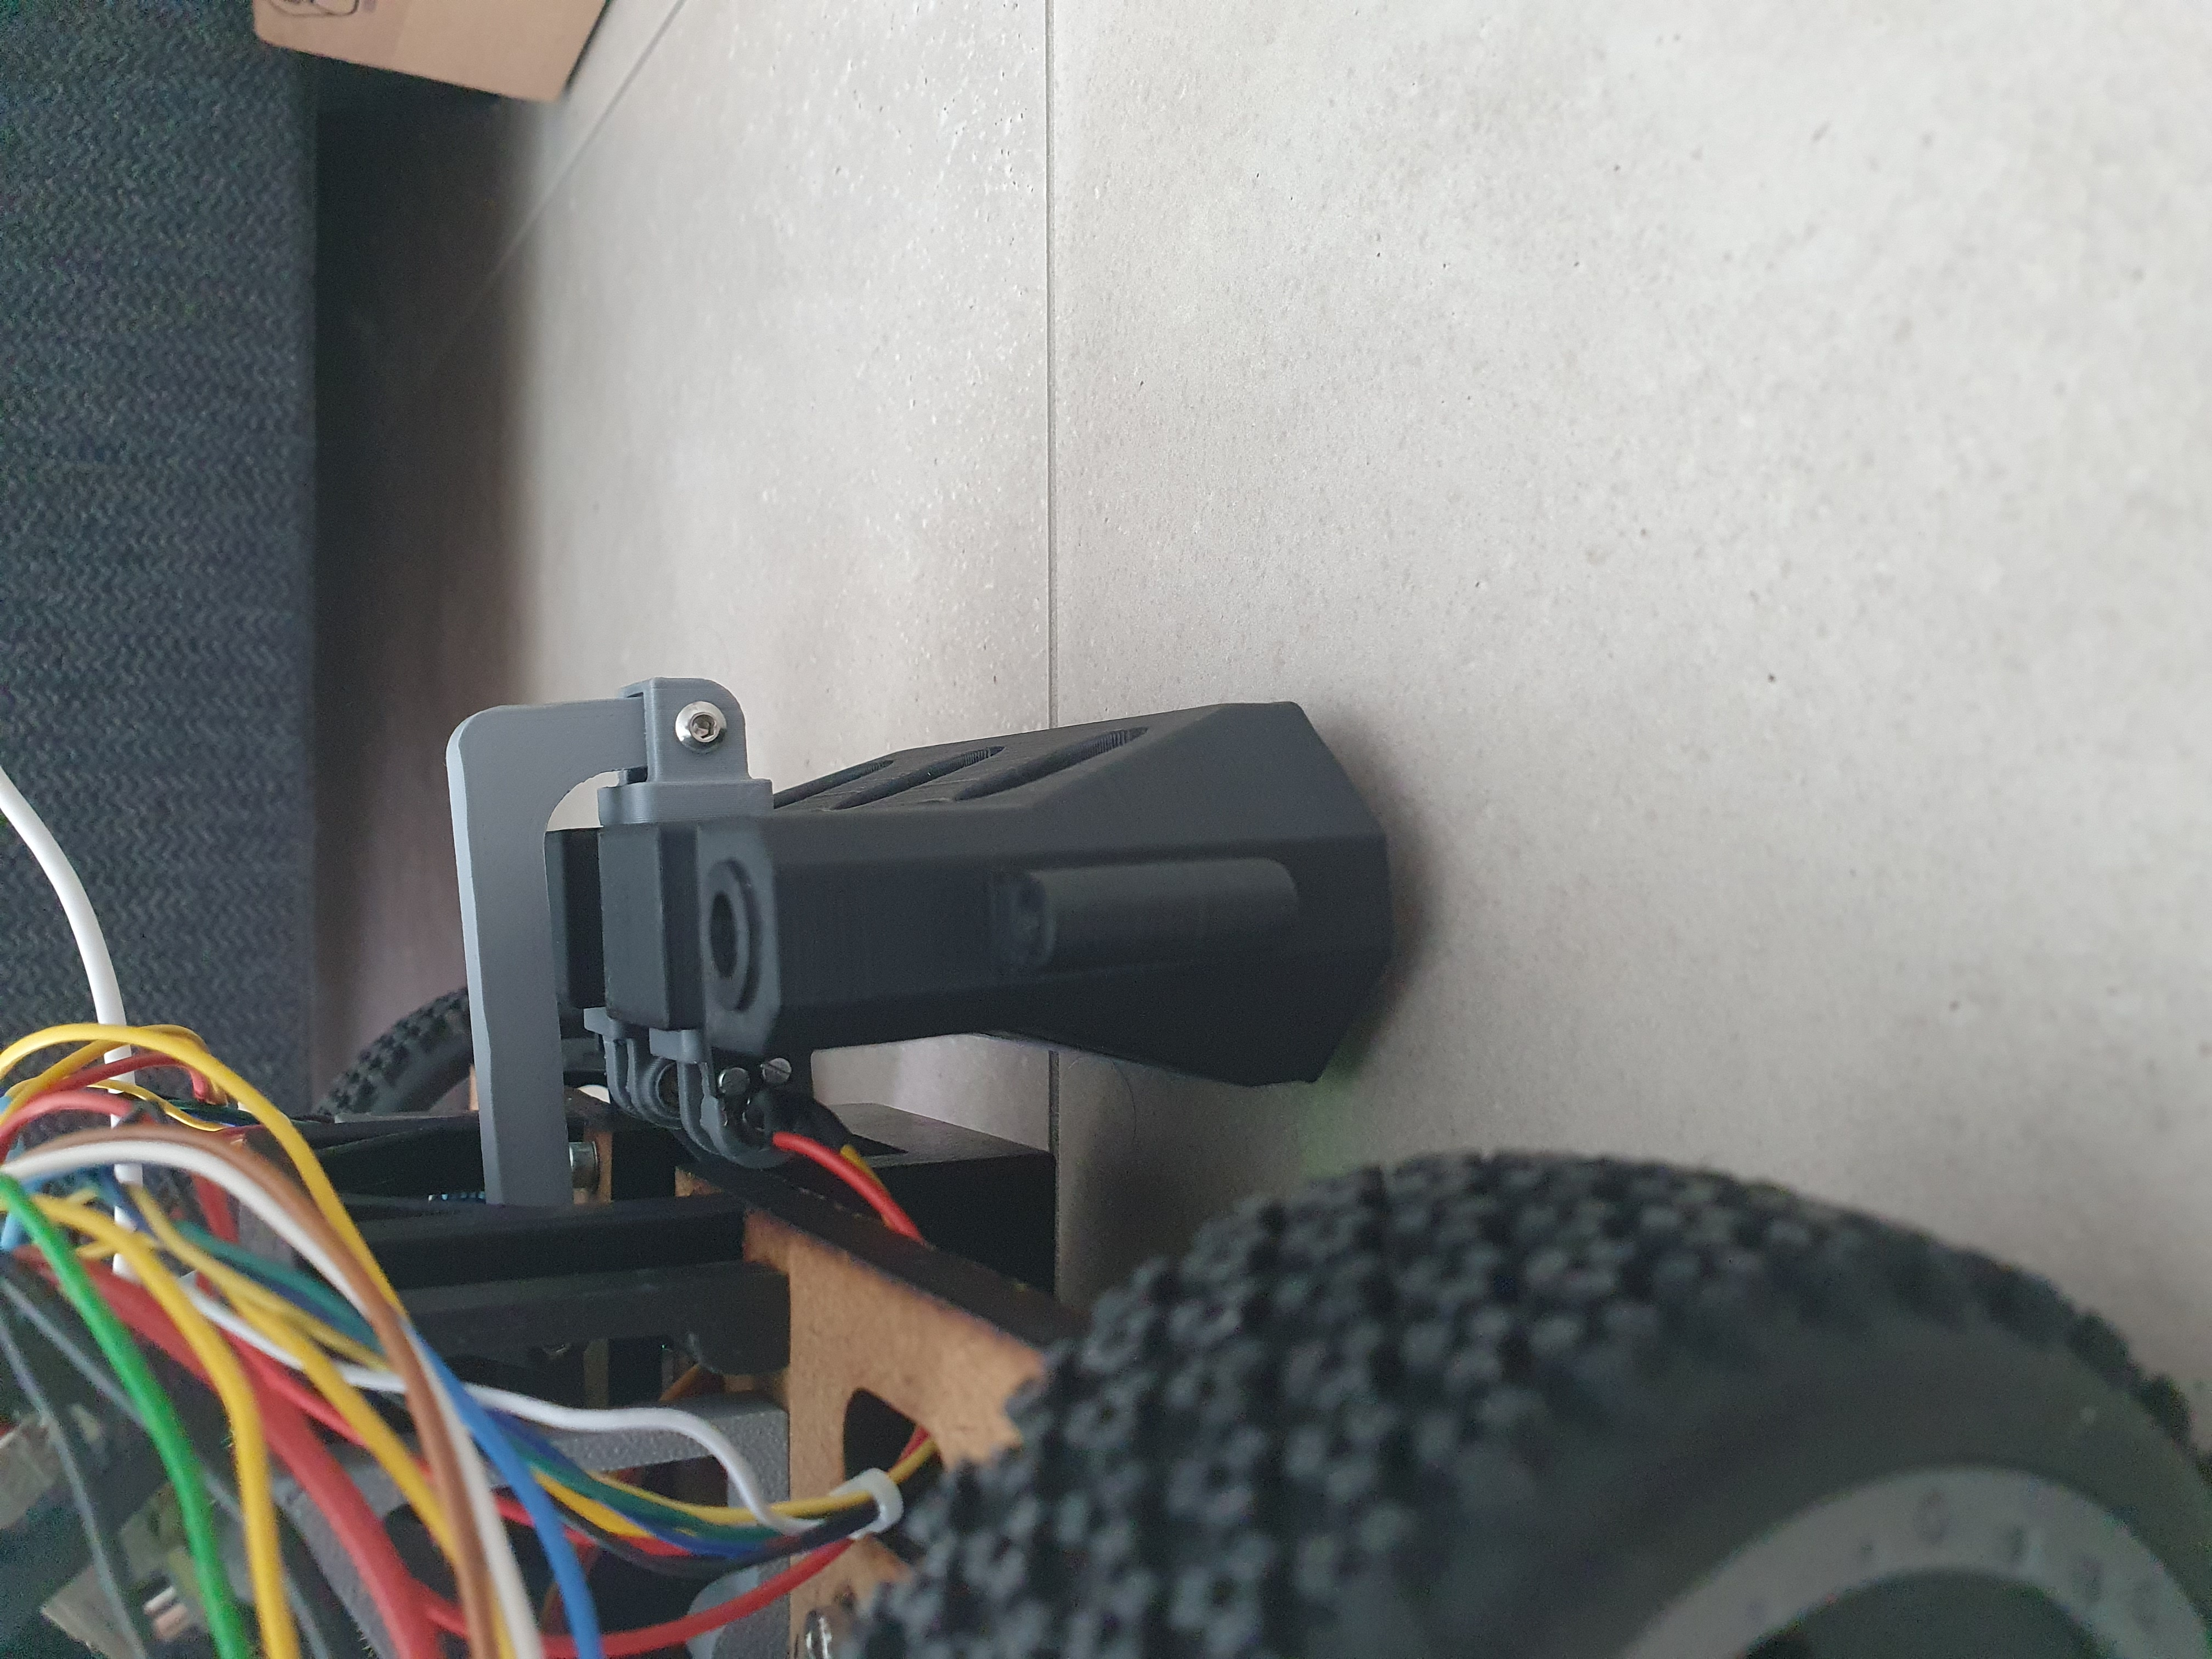
\includegraphics[width=\textwidth, angle=-90]{assets/MT/greifer-close.jpg}
  \caption{Greifer geschlossen}
  \label{fig:griefe-rclose1}
\end{minipage}
\end{figure}
\subsubsection{Wegstellbefehl}

Der Ablauf des Beseitigen eines Hindernisses ist in folgendem Text erklaert und auf der folgenden Grafik \ref{fig:wegstellbefehl} bildlich aufgezeigt.

Falls der Roboter sich noch auf dem vorherigen Knoten befindet und die Kamera die Barriere erkannt hat, fährt er soweit, bis der Ultraschall die Barriere bemerkt auf 7cm Abstand. 
Falls die Kamera keine Barriere im Voraus erkennt und der Ultraschall ein Objekt, das als Barriere erkannt wird, erkennt, hält der Roboter ebenfalls 10cm zuvor.

Dann dreht das Fahrzeug sich um und fährt rückwärts auf die Barriere zu, bis der Endschalter am Greifer betätigt wird. Bei Betätigung wird das Fahrzeug gestoppt und der Greifer hebt das Hindernis an.
Nach dem erfolgreichen Anheben des Objekts, dreht sich das Fahrzeug zurück in seine ursprüngliche Ausrichtung. Anschliessend erfolgt eine Nachkorrektur der Position, um das Objekt wieder an derselben Position abzusetzen.

Der Wert der Nachkorrektur ist 12cm und wurde experimentell ermittelt. Diese Experimente sind im Anhang im Kapitel \nameref{hindernis-nachkorrektur} zu finden.

Nach der Nachkorrektur stellt der Roboter das Hindernis wieder ab und fährt, bis der nächste Knoten erkannt wird.

\begin{figure}[H]
    \centering
    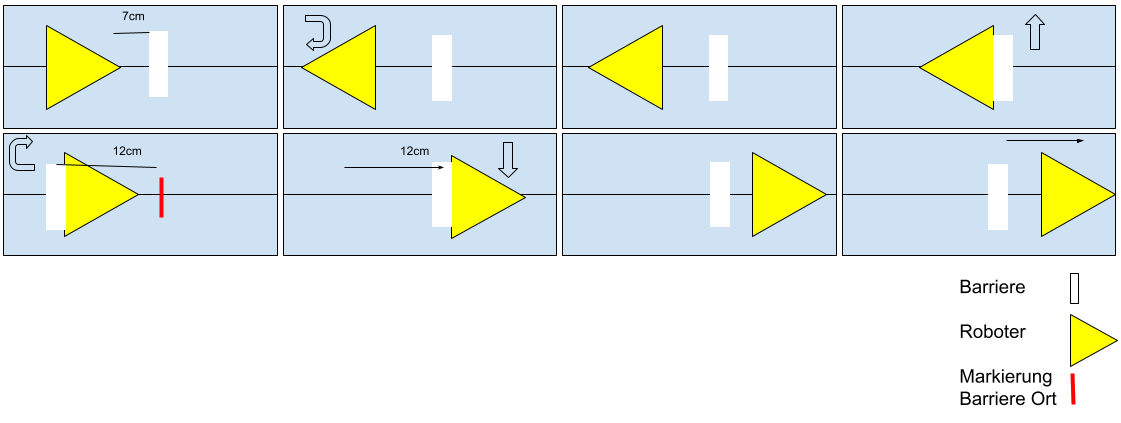
\includegraphics[width=\linewidth]{assets/ET/wegstellbefehl.png}
    \caption{Prozess Wegstellbefehl}
    \label{fig:wegstellbefehl}
\end{figure}


\newpage
%%%%%%%%%%%%%%%%%Epic 6%%%%%%%%%%%%%%%%%%%%%%%%%%%%%%%%%%%%%%%%%%%%%%%%%%%%%%%
\subsection{Auf Linie ausrichten}



\subsubsection{Ausgehende Linien erkennen}
\label{outgoing-lines}

Die eigenständige Software zum Erkennen ausgehender Linien wurde bereits in \acrshort{pren1} umgesetzt und getestet. In \acrshort{pren2} wurde diese Funktionalität in die zentrale Roboter-Software integriert. Abbildung \ref{fig:angle-reader-classdiagramm} zeigt das Klassendiagramm der dafür verantwortlichen Klasse \verb|AngleReader|.

\begin{figure}[H]
    \centering
    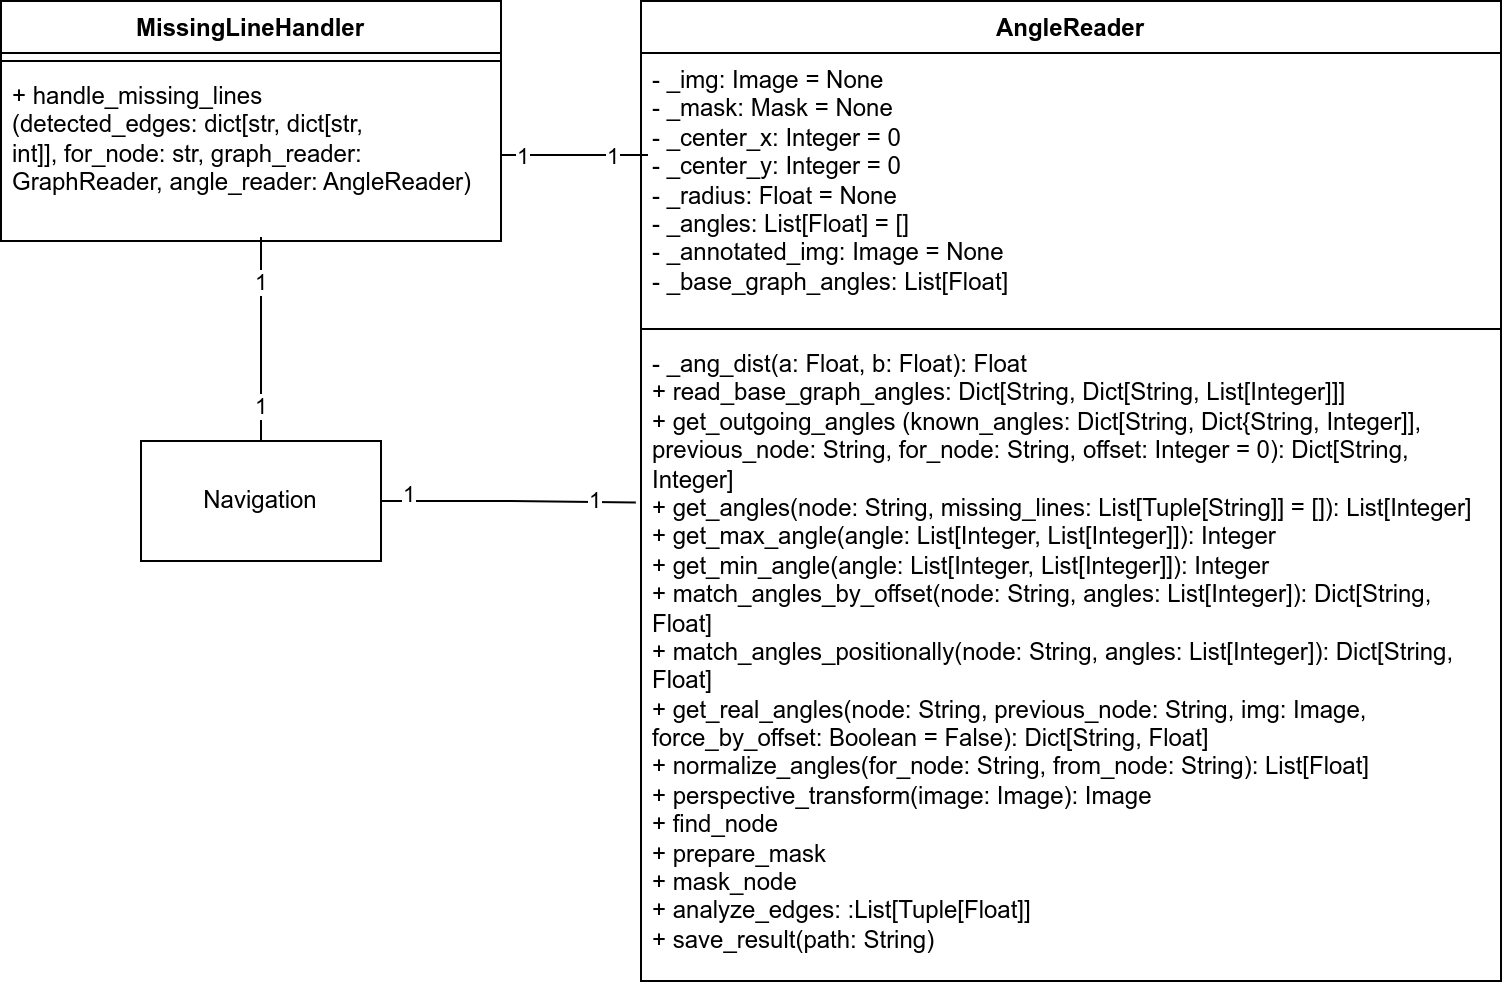
\includegraphics[width=1\linewidth]{assets/IT/robot-sw-architecture-node_reader_angles.png}
    \caption{Angle-Reader Klassendiagramm}
    \label{fig:angle-reader-classdiagramm}
\end{figure}

Die Klasse \verb|AngleReader| ist verantwortlich für das Erkennen und Zuordnen der ausgehenden Kanten eines Knotens anhand eines Bildes. Dabei kommen verschiedene Bildverarbeitungsschritte zum Einsatz: 
\begin{itemize}
    \item Perspektivtransformation zur Normalisierung der Bildansicht
    \item Erkennung des zentralen Knotens (Kreisform) mittels \verb|HoughCircles|
    \item Farbsegmentierung zur Isolation der Linien (Kanten)
    \item Analyse der Konturen zur Berechnung der Winkel der Linien relativ zur Knotenmitte
\end{itemize}

Die detektierten Winkel werden anschliessend mit den erwarteten Winkeln aus einer statischen YAML-Konfigurationsdatei (\verb|base_graph_angles.yml|) abgeglichen. Dies geschieht entweder über:
\begin{itemize}
    \item \textbf{Positionsbasiertes Matching}: Falls die Anzahl erkannter Linien mit der Anzahl erwarteter Linien übereinstimmt, werden die Winkel einfach nach ihrer Reihenfolge im Uhrzeigersinn zugeordnet.
    \item \textbf{Toleranz-basiertes Matching}: Falls eine oder mehrere Linie zu wenig erkannt wurden, wird versucht, die Winkel anhand eines bekannten Winkelbereichs (z.B. $60^\circ \pm 30^\circ$) zuzuordnen.
\end{itemize}

Die Klasse bietet zudem die Möglichkeit, das erkannte Ergebnis mit Winkeln und Konturen auf dem Originalbild zu annotieren und zu speichern, was die Debugging-Möglichkeiten deutlich verbessert. Eine Beispiel Ausgabe vom Knoten E ist in der nachfolgenden Abbildung \ref{fig:angle-reader-debug-output} ersichtlich.

\begin{figure}[H]
    \centering
    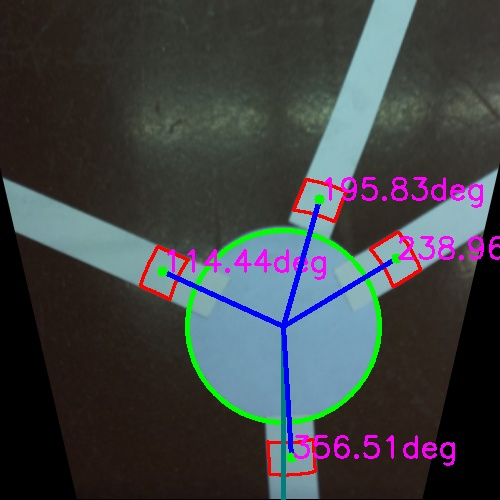
\includegraphics[width=0.5\linewidth]{assets/IT/250525_204610_test_annotated_angles_of_E.jpg}
    \caption{Debugging Ausgabe der Winkelerkennung vom Knoten E}
    \label{fig:angle-reader-debug-output}
\end{figure}

Die Winkel der ausgehenden Linien koennen sehr genau gemessen werden. Dies hilft dem Liniensensor, sobald der Roboter weiterfahren kann. Der Roboter wird sehr genau ausgerichtet, dies hilft dabei, die Linie zu finden und nicht moeglicherweise eine Bodenfuge als Linie zu erkennen. Damit wird Risiko 5 (Bodenfugen als Linie gedeutet) mitigiert.

\textbf{Fehlende Linien erkennen und darauf reagieren}

Falls kein Knoten, zu viele Knoten, oder Kanten oder Kanten in falschen Winkelbereichen detektiert werden, wird folgender mehrstufiger Mechanismus aktiviert, um ein fehlerhaftes Einlesen auszuschliessen, und den Prozess der Winkelerkennung zu wiederholen:
\begin{enumerate}
    \item Der Roboter fährt 20cm zurück.
    \item Danach fährt er in kleinen Schritten vorwärts und macht dabei fortlaufend Bilder, um die Kanten erneut zu erkennen.
    \item Wird auch nach mehreren Versuchen keine vollständige Kantenstruktur erkannt, geht der Roboter davon aus, dass der Knoten nicht vollständig zugänglich oder die Markierungen beschädigt sind, oder er sich verirrt hat, also nicht auf einem Knoten steht, den er erwartet hat. (z.B. Beim traversieren einmal falsch abgebogen.)
    \item In diesem Fall wird der Knoten aus dem internen Graphen entfernt, der Roboter fährt zum vorherigen Knoten zurück und wählt eine alternative Route.
\end{enumerate}
